\section{Experiments}
\label{sec:experiments}
We implemented and trained our SAMNet model using MI-Prometheus~\cite{kornuta2018accelerating}, a framework based on Pytorch~\cite{paszke2017automatic}. We evaluated the model on the COG dataset~\cite{yang2018dataset}, a video reasoning~\cite{mogadala2019trends} dataset developed for the purpose of research on relational and temporal reasoning, as well as on the CLEVR dataset~\cite{johnson2017clevr}, created for Image Question Answering research.
Our experiments were designed to study SAMNet's performance as well as its generalization abilities in different settings.
For the temporal and feature transfer experiments, we used two variants of both datasets.
For COG, an easy one (Canonical) and a Hard variant, differ mainly on the number of frames in the input sequence and number of distractors. See \Sec{sec:temporal} for more information.
For CLEVR, we consider the CoGenT (Constrained Generalization Test) variant which contains two conditions, differing on the combinations of attributes values. See \Sec{sec:feature} for additional details.
For the reasoning transfer experiments, we consider 22 classification tasks in COG and the 5 original question categories in CLEVR.
%More details on the composition of these datasets is available in Appendix \ref{sec:datasets-desc}.

\subsection{Performance comparison with the COG baseline}
\label{sec:cog-baseline-compare}

We trained SAMNet using 8 reasoning steps and external memory of 8 128-floats address locations.
%We have also carried out experiments with different numbers of reasoning steps and memory size, but this goes beyond the scope of this paper.
We focused on 22 classification tasks and compared our results with the baseline model.
The most important results are highlighted in~\cref{fig:samnet_cog_detailed}; full comparison can be found in the supplementary material.%Appendix~\ref{sec:cog-all-results}.

\begin{figure*}[htb]
	\centering
	\begin{subfigure}{\textwidth}
		\centering
		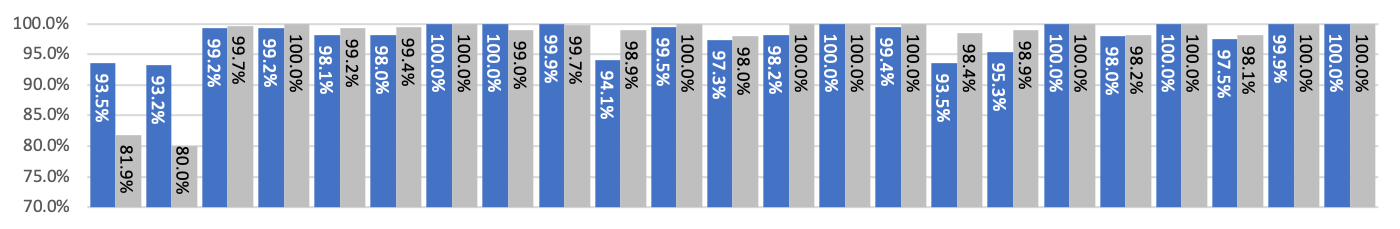
\includegraphics[width=0.9\textwidth]{img/results/samnet_cog_orig_canonical_no_labels.png}
	\end{subfigure}%
	\newline
	\begin{subfigure}{\textwidth}
		\centering
		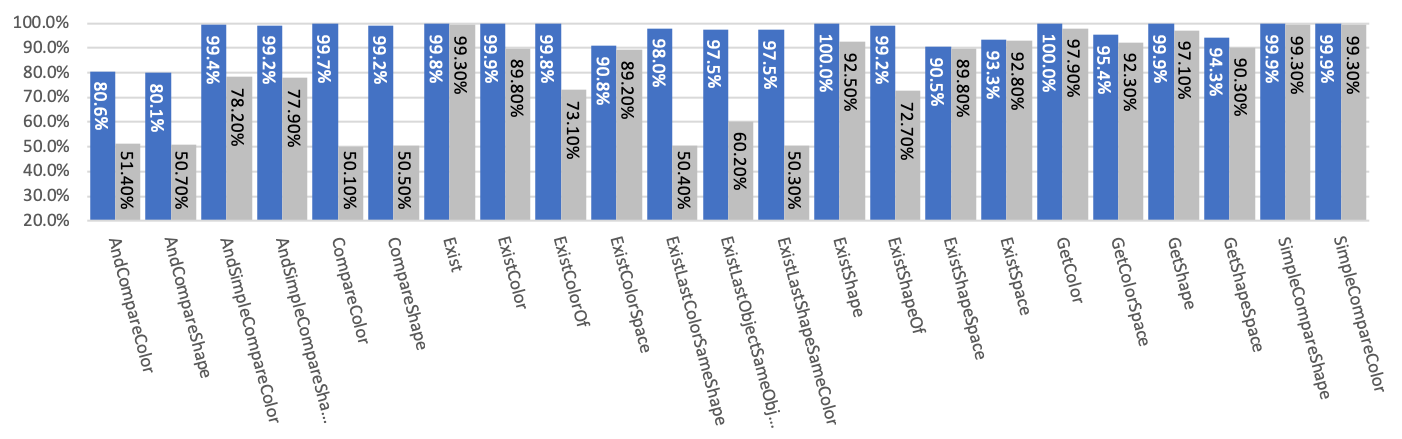
\includegraphics[width=0.9\textwidth]{img/results/samnet_cog_orig_hard.png}
	\end{subfigure}%
	\caption{Comparison of test set accuracies of SAMNet (blue) with original results achieved by the COG model (gray) on Canonical (top) and Hard (bottom) variants of the COG dataset.}
	\label{fig:samnet_cog_detailed}
\end{figure*}

For the Canonical variant (top row), we achieve similar accuracies for the majority of tasks (with a total average accuracy of 98.0\%, compared to 97.6\% for the COG model), with significant improvements (around 13 points) for \textit{AndCompare} tasks.
As these tasks focus on compositional questions referring to two objects, we hypothesize that our model achieves better accuracy due to its ability to selectively pick and store relevant objects from the past frames in memory.
Despite there being some tasks in which our model reached slightly lower accuracies,
% (between 0.2 and 1.8 points)
when comparing performances on the Hard variant, it improves upon the COG baseline on all tasks, with improvements varying from 0.5 to more than 30 points.

\subsection{Reasoning transfer on CLEVR and COG}
\label{sec:reasoning}
In these experiments, we focus on analyzing the impact of each task relatively to others when training jointly.

\subsubsection{CLEVR}
\label{sec:reasoning-clevr}
For the CLEVR dataset, we consider the question categories defined by the authors: \textit{Exist}, \textit{Count}, \textit{CompareInteger}, \textit{CompareAttribute}, \textit{QueryAttribute} and conducted the following experiments:
\begin{itemize}
	\compresslist
	\item Train and test SAMNet on a single task group $t$. These 5 experiments fit into the traditional Deep Learning procedure of single-task learning,
	\item Train SAMNet on all task groups jointly, and evaluate its performance on each task $t$ separately,
	\item Finally, for each task group $t$, we train SAMNet on all tasks but $t$, and test its performance on $t$. %These experiments steer away from single / multi-task training and rather fall under the Domain Adaptation setting, categorized as \emph{transductive} transfer learning in \cite{pan2009survey}.
\end{itemize}

Noticeable results are shown in \Fig{fig:CoGenT-results}, while the complete set is available in the supplementary material.%Appendix \ref{sec:full-cogent-results}.


Looking at \Fig{fig:CoGenT-results}, SAMNet does well on \textit{Count} and \textit{QueryAttribute}, but poorer on the 3 other tasks in the single-task learning setting (dark blue). Indeed, \textit{Exist}, \textit{CompareInteger} and \textit{CompareInteger} are binary tasks; \textit{Count} has for corresponding labels the digits 0 through 10 (a random agent would thus obtain $<$10\% accuracy) and \textit{QueryAttribute} maps to the set of object attributes values (15 labels).

Nevertheless, significant accuracy gains are noted when training jointly on all tasks (light gray), ranging from 18 points to 37 points on 4 out of 5 tasks. \textit{QueryAttribute} only sees an increase of one point. One could qualify it as \textit{self-sufficient} as it does not appear to benefit from joint training with other tasks. These improvements suggest that related tasks benefit from joint training.
We plan to run additional experiments to jointly train on $t$ and all possible subsets of the remaining 4 tasks ($2^4$ experiments per task). We hypothesize that the improvements on e.g. \textit{Exist} would mostly originate from training jointly on \textit{CompareAttribute} and \textit{CompareInteger} since all 3 tasks share the same output space (i.e., labels domain).

Finally, the "all-tasks-but-$t$" experiments (cyan) demonstrate that while tasks are related, one does not subsume another in terms of learning. Indeed, we can observe that for \textit{CompareAttribute}, while \textit{Exist} and \textit{CompareInteger} share the same output space, including them and holding out \textit{CompareAttribute} from the training set results in poor accuracy. We also observe no learning for \textit{Count} and \textit{QueryAttribute}, caused by these tasks having distinct labels domains, which do not overlap with the other tasks. Thus, if holding out samples from \textit{Count} during training, a model will not be able to predict the corresponding labels.

\begin{figure}[!t]
	\centering
	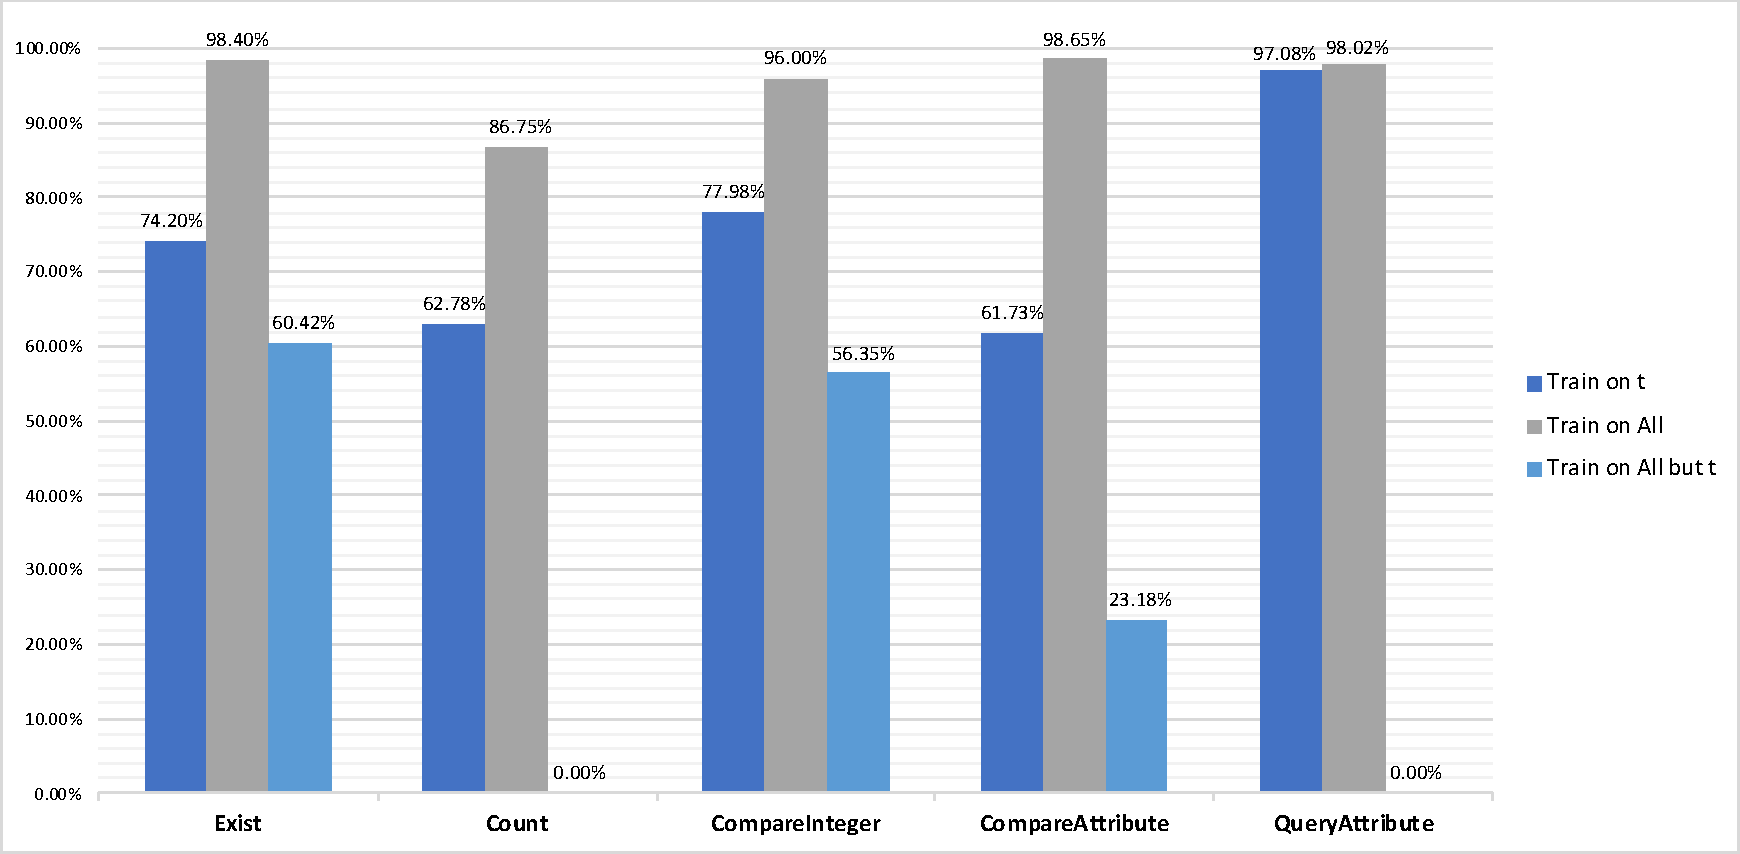
\includegraphics[width=0.5\textwidth]{img/results/CoGenT_results.pdf}
	\caption{CLEVR-CoGenT accuracies for all tasks $t$ when training on $t$ only, training on all tasks jointly and training on all tasks but $t$.} %For all experiments, the validation and test sets are identical.
	\label{fig:CoGenT-results}
\end{figure}

An supplementary set of experiments, for which results are available in the supplementary material,
%Appendix \ref{sec:full-cogent-results}
finetune the model trained on all tasks on each task $t$ respectively. Given the initial training on all tasks, we were interested in the tradeoff between the performance gain, if any, on the finetuned task and the drop, if any, on other tasks. Finetuning did not demonstrate a clear benefit (except for \textit{Count}, where the accuracy increased by 1.5 pt) without hurting performance on the other tasks. Nevertheless, these experiments leave open the possibility that the multi-task learning training method may potentially benefit from using weighted sampling towards the tail end with more emphasis on samples from less performing task groups. Recent work~\cite{guo2018dynamic, kendall2018multi} in this direction has been done, although seems to weigh tasks rather than samples.

\subsubsection{COG}
\label{sec:reasoning-cog}
\tsj{todo}


\subsection{Temporal transfer on COG}
\label{sec:temporal}


The goal here is to test the generalization ability concerning the sequence length and number of distractors.
For that purpose, we compare both models when trained on the Canonical variant and tested on Hard (\cref{fig:samnet_cog_overall_transfer}).

\begin{table}[ht]
	\centering
	\begin{adjustbox}{width=0.45\textwidth}
		\begin{tabular}{lccc}
			\toprule
			Variant	&	Number of frames	&	Max. memory duration	&	Max. number of distractors \\ 
			\midrule
			Canonical & 4 & 3 & 1\\	
			Hard  & 8 & 7 & 10\\
			\bottomrule	
		\end{tabular}
	\end{adjustbox}
	\caption{Details of the Canonical and Hard variants of the COG dataset.}
	\label{tab:cog_variants}
\end{table}\vspace{5pt}

As the original paper does not include these experiments, we performed them. The light gray color indicates original results, whereas dark gray indicates the accuracies of COG models which we trained (fine-tuning/testing) using the original code provided by the authors.
For sanity check, in the first column, we report both the best-achieved score and the score reported in the paper when training and testing on the Canonical variant, without any fine-tuning. The observed close scores underline the faithfulness of the model reproducibility.
In a pure \textit{zero-shot learning} setup (second column), our model shows enormous generalization ability, reaching 91.6\% accuracy on the test set.
We also test both models in a setup where the model trained on a Canonical variant underwent additional fine-tuning (for a single epoch) on the Hard variant (third column).
In this case, the SAMNet model again reaches exemplary performance, at 96.7\% accuracy, and, interestingly, performs better than the model trained solely on the Hard variant.

\begin{figure}[htb]
	\centering
	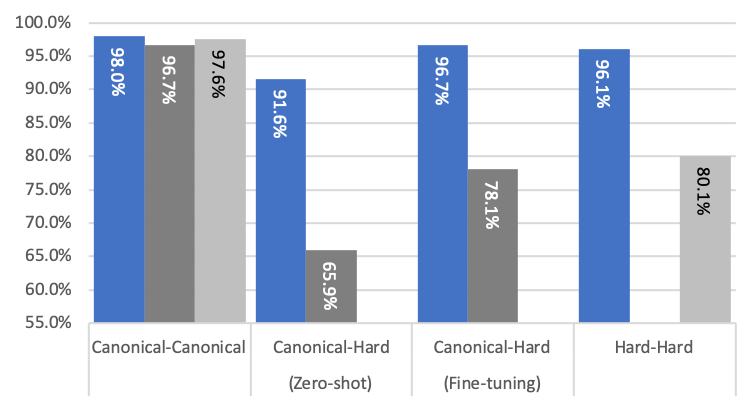
\includegraphics[width=0.5\textwidth]{img/results/samnet_cog_overall_transfer.png}
	\caption{Total accuracies of SAMNet (blue) and COG models (light/dark gray) when testing generalization from Canonical to Hard variants of the dataset.}
	\label{fig:samnet_cog_overall_transfer}
\end{figure}


\subsection{Feature transfer on CLEVR-CoGenT}
\label{sec:feature}
\begin{table}[ht]
	\label{tab:cogent_conditions}
	\centering
	\begin{adjustbox}{width=0.45\textwidth}
		\begin{tabular}{cccc}
			\toprule
			Dataset	& Cubes	& Cylinders &	Spheres	\\
			\midrule
			CoGenT A & Gray / Blue / Brown / Yellow  & Red / Green / Purple / Cyan	&	Any color  \\
			CoGenT B	&	Red / Green / Purple / Cyan &	Gray / Blue / Brown / Yellow	&	Any color \\
			\bottomrule
		\end{tabular}
	\end{adjustbox}
	\caption{Colors \& shapes combinations present in CoGenT-A \& -B datasets.}
\end{table}

The final set of experiments we consider is related to domain adaptation. %According to \cite{pan2009survey}, this settings considers different but related source and target domains, under a common task.

The CoGenT-A \& -B sets of CLEVR differ by the available combinations of object attributes (\Tab{tab:cogent_conditions}). If we consider the input domain to be the set of objects with all attributes values, both sets differ by the data distribution they are sampled from. We thus consider 2 experiments with SAMNet trained on CoGenT-A: A direct generalization test (\emph{zero-shot learning}) from A to B and a finetuning of a single epoch on 30k Conditions B samples (following the procedure of~\cite{johnson2017inferring, mascharka2018transparency, perez2018film, marois2018transfer}. The results are available in \Fig{fig:CoGenT-B-results}.

\begin{figure}[!t]\vspace{5pt}
	\centering
	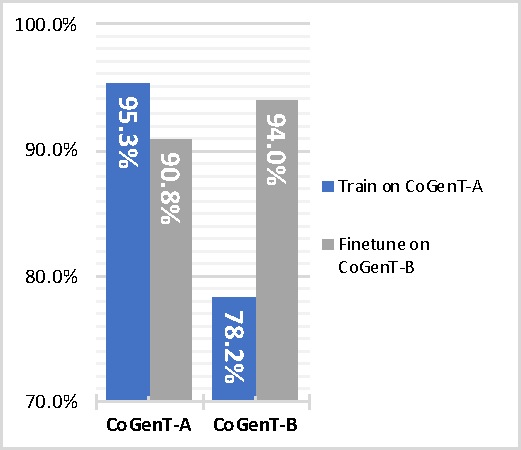
\includegraphics[width=0.3\textwidth]{img/results/CoGenT_B_results.pdf}
	\caption{CLEVR-CoGenT accuracies for all tasks $t$ when training on $t$ only, training on all tasks jointly and training on all tasks but $t$.} %For all experiments, the validation and test sets are identical.}
	\label{fig:CoGenT-B-results}
\end{figure}
Evaluating SAMNet on CoGenT shows that performance is worse on CoGenT-B than CoGenT-A, in line with~\cite{johnson2017inferring, mascharka2018transparency, perez2018film}. Finetuning for a single epoch allows an observable increase of 15 pts on CoGenT-B, and a slight drop on CoGenT-A, also observed in other models.